[2~v\textsuperscript{o}]
C'est donc \`{a} cet egard
\edtext{que les pointes receuuront}{\lemma{que}\Bfootnote{%
\textit{(1)}\ la pointe %
\textit{(2)}\ les pointes %
\textit{(a)}\ auront %
\textit{(b)}\ receuuront \textit{L}}}
tousjours le m\^{e}me
\edtext{pli, pour}{\lemma{pli,}\Bfootnote{\textit{(1)}\ de \textit{(2)}\ pour \textit{L}}}
le mouuement ou passage du mobile.
Or \edtext{un m\^{e}me ressort\protect\index{Sachverzeichnis}{ressort}}{\lemma{}\Bfootnote{un\ \textbar\ m\^{e}me \textit{erg.}\ \textbar\ ressort \textit{L}}}
\edtext{ou egal}{\lemma{}\Bfootnote{ou egal \textit{erg. L}}}
receuuant tousjours un m\^{e}me pli, re\c{c}oit
tousjours une m\^{e}me
force\protect\index{Sachverzeichnis}{force}.
Donc le mobile $\displaystyle M$, quelle
vistesse\protect\index{Sachverzeichnis}{vitesse}
qu'il puisse avoir, perdra tousjours une
\edtext{m\^{e}me quantit\'{e} de force}{\lemma{m\^{e}me}\Bfootnote{\textit{(1)}\ force \textit{(2)}\ quantit\'{e} de force, \textit{L}}},
et par consequent,
(puisque son corps demeure le m\^{e}me)
un m\^{e}me degrez de vistesse.
\pend
\pstart
Ainsi supposant la surface $\displaystyle AB$
\edtext{ou le lieu o\`{u} le mobile passe}{\lemma{}\Bfootnote{ou le [...] passe \textit{erg. L}}}
\edtext{parsem\'{e} egalement de distance en distance}{\lemma{parsem\'{e}}\Bfootnote{\textit{(1)}\ par tout \textit{(2)}\ egalement [...] en distance \textit{L}}}
de semblables pointes
\edtext{d'egale force}{\lemma{}\Bfootnote{d'egale force \textit{erg. L}}}\edtext{;
le lieu retardera par tout \'{e}galement le mobile,
et deminuera tousjours son mouuement d'un m\^{e}me
degrez de vitesse\protect\index{Sachverzeichnis}{degr\'{e} de vitesse},
et par consequent les theoremes que j'ay traittez auront lieu.}{\lemma{force;}\Bfootnote{\textit{(1)}\ les\
\textit{(a)}\ diminuitions\
\textit{(b)}\ pertes des vitesses \`{a} cet egard seront proportionelles aux
espaces parcourus\protect\index{Sachverzeichnis}{espace parcouru}
de la maniere que je viens d'expliquer
\textit{(2)}\ elle
\textit{(3)}\ elle retardera par tout \'{e}galement
\textit{(4)}\ le lieu ou
\textit{(5)}\ le lieu [...] \'{e}galement\
\textit{(a)}\ la vi\
\textit{(b)}\ le mobile,\
\textit{(aa)}\ et que\
\textit{(bb)}\ sans avoir \'{e}gard\
\textit{(cc)}\ et deminuera\
\textit{(aaa)}\ sa vitesse\
\textit{(bbb)}\ tousjours [...] theoremes\
\textit{(aaaa)}\ susdits\
\textit{(bbbb)}\ que [...] lieu.
\textit{L}}}
\pend
\count\Bfootins=1000
\pstart
Il est vray pourtant que la
Resistence respective\protect\index{Sachverzeichnis}{r\'{e}sistance respective}
est compliqu\'{e}e
\edtext{dans le frottement}{\lemma{}\Bfootnote{dans le frottement \textit{erg. L}}}
avec la
Resistence absolue\protect\index{Sachverzeichnis}{r\'{e}sistance absolue}.
Car \edtext{imaginons la surface $\displaystyle AB$ comme perc\'{e}e en sorte que}{\lemma{imaginons}\Bfootnote{\textit{(1)}\ que
\textit{(2)}\ la surface [...] sorte que
\textit{L}}}
la \edtext{pointe $\displaystyle P$ ne puisse seulement luy devenir parallele, estant pli\'{e}e en $\displaystyle p$,
mais qu'elle puisse m\^{e}me aller}{\lemma{pointe}\Bfootnote{%
\textit{(1)}\ $\displaystyle CP$ %
\textit{(2)}\ $\displaystyle P$ %
\textit{(a)}\ ne puisse seulement luy devenir parallele, estant pli\'{e}e, en $\displaystyle p$ mais aller m\^{e}me auss %
\textit{(b)}\ pli\'{e}e par le mobile puis %
\textit{(c)}\ ne puisse [...] aller %
\textit{L}}}
au dessous de la surface
\edtext{jusqu'\`{a} $\pi$}{\lemma{jusqu'\`{a} }\Bfootnote{\textit{(1)}\ $\displaystyle C$
\textit{(2)}\ $\pi$.
\textit{L}}}.
Cela pos\'{e} il est asseur\'{e}, qu'elle sera pouss\'{e}e d'autant plus loin,
que \edtext{le mouuement du mobile}{\lemma{le}\Bfootnote{\textit{(1)}\ mobile
\textit{(2)}\ mouuement du mobile
\textit{L}}}
$\displaystyle M$ sera plus viste,
et qu'ainsi \`{a} l'\'{e}gard de ce pli
\edtext{superflu du ressort}{\lemma{superflu}\Bfootnote{\textit{(1)}\ du dit ressort
\textit{(2)}\ du ressort
\textit{L}}}
qui fait la pointe
\edtext{$\displaystyle P$}{\lemma{}\Bfootnote{ \textit{$\displaystyle P$ erg. L}}}
le mobile perdra d'autant plus de force, qu'il va avec plus de vistesse.
Parce qu'il communique plus de force au ressort qu'il plie d'avantage.
Et \edtext{cela est vray}{\lemma{cela}\Bfootnote{\textit{(1)}\ vray
\textit{(2)}\ est vray,
\textit{L}}},
quoyque la surface
\edtext{$\displaystyle AB$}{\lemma{$\displaystyle AB$}\Bfootnote{\textit{erg. L}}}
ne soit point
\edtext{perc\'{e}e, et quoyque ce pli superflu jusqu'en $\pi$ ne puisse arriver effectivement, car}{\lemma{perc\'{e}e,}\Bfootnote{\textit{(1)}\ car
\textit{(2)}\ et quoyque [...] superflu\
\textbar\ jusqu'en $\pi$ \textit{erg.}\ \textbar\
ne puisse [...] car
\textit{L}}}
toute la
masse\protect\index{Sachverzeichnis}{masse}
du \edtext{corps dont $\displaystyle AB$ est la surface receuura le choc, et empechera}{\lemma{corps}\Bfootnote{\textit{(1)}\ qui empeche ce
\textit{(2)}\ $\displaystyle AB$
\textit{(3)}\ dont [...] empechera
\textit{L}}}
la pointe $\displaystyle P$ d'aller plus avant qu'en $\displaystyle p$.
Cependant le mobile $\displaystyle M$ ne laissera pas d'avoir perdu autant de force,
que si la
\edtext{pointe $\displaystyle P$ avoit}{\lemma{pointe $\displaystyle P$}\Bfootnote{\textit{(1)}\ auroit
\textit{(2)}\ avoit
\textit{L}}}
pu aller effectivement jusqu'en $\pi$,
puisqu'il luy a donn\'{e} une fois un
choc\protect\index{Sachverzeichnis}{choc}
suffisant pour le faire sans l'obstacle
\edtext{qui en a empech\'{e} l'effect.}{\lemma{qui}\Bfootnote{\textit{(1)}\ est
\textit{(2)}\ s'est trouu\'{e}
\textit{(3)}\ en a empech\'{e} l'effect.
\textit{L}}}\edlabel{035,09,11_002v_Abschr.}
\pend
\newpage
\count\Bfootins=1200
\pstart 
%\vspace{1em} 
\begin{center} [\textit{Teil 3}] \end{center} \pend
\pstart
\noindent
\begin{wrapfigure}[7]{l}{0.28\textwidth}
   \vspace{-4mm}  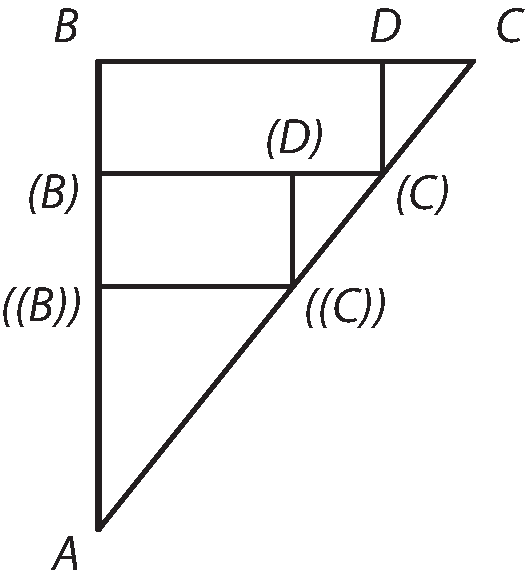
\includegraphics[trim = 0mm 0mm -5mm 0mm, clip, width=0.28\textwidth]{images/lh0350911_002v-d1.pdf}
     \centering
   [\textit{Fig. 4}]% \caption{Bildbeschreibung}
  \end{wrapfigure}
%
In diminutione motus arithmetica secundum loca spatiis 
\edtext{residuis}{\lemma{}\Bfootnote{residuis \textit{erg. L}}}
\edtext{existentibus $\displaystyle AB$,
celeritatum\protect\index{Sachverzeichnis}{celeritas}
imminutiones sunt in reciproca \protect\rule[-4mm]{0mm}{10mm}$\displaystyle CD$ invicem aequales $\displaystyle \frac{a}{b}\beta \, \sqcap \, CD.$
$\displaystyle AB \sqcap x$ spatia residua, $\displaystyle BC \, \sqcap \, \frac{a}{b}x$ celeritates residuae,
$\displaystyle \frac{a^2}{\displaystyle \frac{a}{b}x} \sqcap \frac{ba}{x}$ temporum incrementa:
Et logarithmi erunt ipsa tempora.}{\lemma{existentibus $\displaystyle AB$,}\Bfootnote{\textit{(1)}\ celeritates sunt $\displaystyle BC.$
\textit{(2)}\ celeritatum\protect\index{Sachverzeichnis}{celeritas}
imminutiones sunt\
\textit{(a)}\ $\displaystyle BC.$ sit $\displaystyle AB \, \sqcap \, x.$ erunt et $\displaystyle BC \, \sqcap \, y.$ erit $\displaystyle y \sqcap \frac{a}{b}x$. Temporis autem diminutiones sunt $\displaystyle \frac{a^2}{y}$. Celeritates residuae sunt\
\textit{(aa)}\ $\displaystyle AB$\
\textit{(bb)}\ $\displaystyle \sqcap$ spatia $\displaystyle ABC$, nempe $\displaystyle \frac{a}{2b}x^2$.\
\textit{(aaa)}\ Ergo tempora i\
\textit{(bbb)}\ Jam temporum\
\textit{(aaaa)}\ quibus\
\textit{(bbbb)}\ incrementa sunt\
\textit{(b)}\ in reciproca [...] aequales\
\textit{(aa)}\ celeritates residuae\
\textit{(bb)}\ $\displaystyle \frac{a}{b}\beta \, \sqcap \, CD$. [...] $\displaystyle \frac{a^2}{\displaystyle \frac{a}{b}x} \sqcap \frac{ba}{x}$\
\textit{(aaa)}\ celeritates\
\textit{(bbb)}\ temporum [...] tempora.
\textit{L}}}
Pone $\displaystyle \frac{ba}{x}\, \sqcap\, z.$ fiet $\displaystyle x\, \sqcap\, \frac{ba}{z}.$
\rule[-4mm]{0mm}{10mm}pone $\displaystyle BC\, \sqcap\, c.$ fiet $\displaystyle c\, \sqcap\, \frac{a}{b}x.$ sive $\displaystyle x\, \sqcap\, \frac{b}{a}c$.
Si sit diminutio non celeritatum sed \rule[-4mm]{0mm}{10mm}
\edtext{virium\protect\index{Sachverzeichnis}{vis},
fiet $\displaystyle c \, \sqcap \, a - \sqrt{\protect\vphantom{\protect\mathstrut \frac{a}{b}}} \frac{a}{b}x$ et
$\displaystyle c^2 \! - 2ca + a^2 \sqcap \, \edtext{\frac{\lbrack a \rbrack}{b}x$}{\lemma{}\Bfootnote{$\displaystyle a^2$ \textit{L ändert Hrsg.}}}
}{\lemma{8 \hspace{1.3mm}virium,}\killnumber\Bfootnote{\textit{(1)}\ pro $\displaystyle c$ ponendum est $\displaystyle \frac{c^2}{a}$, et fiet $\displaystyle x \sqcap \frac{b}{a^2}c^2$ et erunt
\textit{(2)}\ fiet $\displaystyle c \, \sqcap \, a - \! \sqrt{\protect\vphantom{\protect\mathstrut \frac{a}{b}}} \frac{a}{b}x$ et\
\textit{(a)}\ $\displaystyle c^2 \! - 2ca + a^2 \sqcap \frac{a^2}{b}x^2$\
\textit{(b)}\ $\displaystyle c^2 \! - 2ca + a^2 \sqcap \, \frac{\lbrack a \rbrack}{b}x$ \textit{L}}}\edtext{incrementa celeritatum}{\lemma{incrementa}\Bfootnote{\textit{(1)}\ virium
\textit{(2)}\ celeritatum
\textit{L}}}
in arithmetica temporum ratione
\edtext{in motu gravium}{\lemma{}\Bfootnote{in motu gravium \textit{erg. L}}}.
Celeritates ut
\edtext{tempora insumta, spatiorum}{\lemma{tempora}\Bfootnote{\textit{(1)}\ spatiorum
\textit{(2)}\ insumta, spatiorum
\textit{L}}}
incrementa, ut celeritates
\edtext{quaesitae}{\lemma{}\Bfootnote{quaesitae \textit{erg. L}}},
ergo ut tempora.
Spatia 
\edtext{percursa in duplicata ratione incrementorum suorum, seu in duplicata ratione celeritatum}{\lemma{percursa in duplicata ratione}\Bfootnote{\textit{(1)}\ celeritatum
\textit{(2)}\ incrementorum [...] celeritatum
\textit{L}}}
quaesitarum vel temporum.
Ergo celeritates quaesitae
\edtext{in subduplicata ratione}{\lemma{in}\Bfootnote{\textit{(1)}\ duplicata ratione
\textit{(2)}\ subduplicata ratione
\textit{L}}}
spatiorum.
Sint spatia $\displaystyle s.$ celeritates $\displaystyle c.$ erit $\displaystyle s \, \sqcap\, \frac{c^2}{b}$.
Ergo $\displaystyle c \, \sqcap\, \sqrt{\vphantom{bs}} bs$.
Jam incrementa celeritatum\protect\index{Sachverzeichnis}{incrementum celeritatis}
$\displaystyle \, \sqcap\ z\, \sqcap\ \sqrt{bs+\beta b} - \sqrt{\mathstrut bs}\, \sqcap\, \beta \sqrt{\vphantom{\mathstrut \frac{b}{x}}} \rule[-4mm]{0mm}{10mm}\frac{b}{x}.$
quae incrementa celeritatum in aequalibus scilicet partibus spatii
\edtext{acquiruntur.}{\lemma{acquiruntur.}\Bfootnote{\
\textbar\ Haec autem incrementa celeritatum in motu per locum retardato sunt decrementa. Ergo celeritates residuae erunt\
\textit{gestr.} \textbar\ \textit{L}}}
\pend
\count\Bfootins=1500
%\newpage
